% !TEX TS-program = xelatex
% == NTI/KAS semestral, téma: Jak získat "kvalitní náhodu". HW zařízení, SW možnosti, dostupné implementace. ==
\documentclass[a4paper,12pt]{article}
% Klasika:
\usepackage[FM,noheader,bw]{tul}
\usepackage{polyglossia}
\setdefaultlanguage{czech}
\usepackage{xevlna}
\usepackage[all]{nowidow}
\finalhyphendemerits=200000
\usepackage[backend=biber, style=iso-numeric]{biblatex}
\addbibresource{zdroje.bib}
\DeclareDelimFormat{finalnamedelim}{\addspace a\space}
% Pomocí \nocite budou zdroje vypsány v seznamu bibliografie bez nutnosti explicitní citace \cite
\nocite{z1,z2,z3,z4,z5,z6}
% Balík TUL bez použití documentclass{tulthesis} neimportuje hyperref (pro funkční odkazy):
\usepackage{hyperref}
\hypersetup{colorlinks=true, linkcolor=tul, urlcolor=tul, citecolor=tul}
% Díky balíku caption kliknutí na \ref odkazující na obrázek skočí na obrázek, a ne na popisek pod ním:
\usepackage{caption}

\begin{document}
	\TULtitlepage{NTI/KAS – semestrální práce:\\Jak získat „kvalitní náhodu“}{Radek Mocek}{29.~listopadu~2024}
	\nofootaddress
	
	\section{Pojmy a upřesnění}
	
	\subsection{Entropie}
	
	Pojem entropie pochází z termodynamiky a obecně značí míru neuspořádanosti. Konkrétněji v oblasti počítačů se jako entropie chápe náhoda získaná z nějakého hardwarového zdroje. Zdrojem entropie může být uživatelská aktivita (např. čas mezi údery do klávesnice, pohyb myši) nebo fyzikální a kvantové děje (např. měření akustického šumu).
	
	\subsection{Generátor náhodných čísel}
	
	Generátory náhodných čísel (RNG) se obecně dělí na hardwarové generátory náhodných čísel (TRNG) a generátory pseudonáhodných čísel (PRNG).
	
	TRNG generují nedeterministické sekvence čísel. Aby generace takových čísel byla možná, musí být součástí TRNG zdroj entropie, který zajišťuje nepředvídatelnost generované sekvence. TRNG jsou ve většině případů pomalejší než PRNG.
	
	PRNG jsou deterministické algoritmy generující sekvence čísel, které se tváří náhodně. Pro stejné startovní podmínky ale PRNG generují stejné výsledky. Jejich podmnožinou jsou pak kryptograficky bezpečné generátory pseudonáhodných čísel (CS-PRNG), které jsou sice deterministické, ale splňují určité předpoklady a díky tomu mohou být použity pro kryptografické účely.
	
	\subsection{Kvalitní náhoda}
	
	Jako „perfektní náhoda“ se často označují sekvence, kde jsou mezi sebou jednotlivé hodnoty nezávislé a všechny mají stejné rozdělení pravděpodobnosti (IID – independent and identically distributed). Fyzikální jevy, jejichž šum se používá jako zdroj entropie, vždy obsahují jistou míru korelace. Proto se často používají tzv. extraktory entropie (\textit{\mbox{randomness} extractor}), což jsou funkce, které částečně entropická data převádějí na data, která se více blíží k IID.
	
	Z důvodu nižší rychlosti TRNG se v reálných nasazeních kombinují oba typy generátorů, kdy je výstup TRNG vstupem do extraktoru entropie a výstup extraktoru je vstupem do CS-PRNG. Tím vzniká systém, který je vhodný pro kryptografické účely, nedeterministický a rychlý (viz obrázek \ref{_tag_img_hybridsystem}).
	
	\begin{figure}[ht]
		\centering
		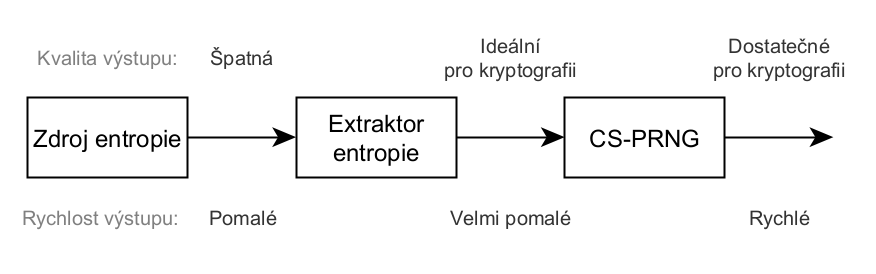
\includegraphics[width=\textwidth]{src/img0}
		\caption{Hybridní RNG systém}
		\label{_tag_img_hybridsystem}
	\end{figure}
	
	Generátory typu PRNG mají svůj vnitřní stav, ze kterého pomocí funkce $f_\mathrm{out}$ vytvoří náhodný výstup. Následně se použije funkce $f_\mathrm{next}$ pro změnu stavu, ze kterého pak může být opět pomocí $f_\mathrm{out}$ vygenerována nová hodnota. Aby byl takový generátor považován za kryptograficky bezpečný, měl by splňovat:
	\begin{itemize}
		\item Těžce invertovatelná $f_\mathrm{out}$: Se znalostí výstupních bitů by nemělo být možné zjistit hodnotu vnitřního stavu generátoru.
		\item Těžce invertovatelná $f_\mathrm{next}$ (\textit{backtracking resistance}): Pokud útočník zjistí vnitřní stav, může aplikováním $f_\mathrm{next}$ zjistit stavy budoucí. Útočník by ale neměl být schopen zjistit stavy předcházející.
		\item Nepředvídatelný budoucí stav (\textit{forward prediction resistance}): Útočník by u generátoru s touto vlastností neměl být schopen ze zjištěného stavu odvodit ani stavy budoucí. V takovém případě musí být vstupem $f_\mathrm{next}$ kromě aktuálního stavu také nově vygenerovaná entropická data. Tato vlastnost bývá označována jako dobrovolná a nesplňují ji všechny CS-PRNG.
	\end{itemize}
	
	\section{Hardware TRNG}
	
	\subsection{Elektronický šum}
	
	Používaným zdrojem entropie je elektronický šum, který se dále dělí (mimo jiné) na tepelný, výstřelový a kmitavý šum. Tepelný šum se vyskytuje ve všech elektronických zařízeních s nějakým odporem (např. diody, triody, MOSFET) a vzniká tepelným pohybem elektronů. Tepelný šum je bílý, což je vhodné pro použití jako zdroj entropie.	Výstřelový šum je způsoben tokem elektrického náboje. Oproti tepelnému šumu se tedy vyskytuje ve vodiči jen tehdy, když je vodič připojený ke zdroji napětí a protéká jím proud. Výstřelový šum je také bílý. Kmitavý šum je růžový a vzniká v oblasti PN přechodu z důvodu nedokonalostí součástek.
	
	Z elektronického šumu tedy lze vytvářet náhodné posloupnosti bitů. Generátory tohoto typu jsou obvykle vybaveny operačním zesilovačem, protože amplituda šumu je nižší než amplituda výstupu TRNG. Použití operačního zesilovače znamená větší spotřebu energie a plochy. Pro převod šumu na diskrétní hodnoty se používá buď analogově-digitální převodník, nebo time-to-digital převodník (TDC).
	
	\subsection{Chaotický systém}
	
	Zdrojem entropie může být také obvod realizující chaotický systém. Výstup takového obvodu je sice deterministický, ale velmi citlivý na počáteční podmínky. Pokud je na vstup chaotického systému poslána např. hodnota elektronického šumu, pak bude jeho výstup dlouhodobě nepředvídatelný. Logiku chaotického systému lze realizovat zcela digitálně např. pomocí rychlého hradlového pole.
	
	\subsection{Jitter}
	
	V logických obvodech se rozdíl mezi hodinovým signálem a signálů z něj odvozených nazývá jitter a lze jej použít jako zdroj entropie. Pro jeho realizaci se v návrzích TRNG používají kruhové oscilátory (viz obrázek \ref{_tag_img_jitter}). Namísto klopného obvodu lze také použít převodník TDC, který převádí vzdálenosti mezi hranami signálu na binární data.
	
	Kruhové oscilátory jsou jednoduché na implementaci, ale mají dva nedostatky. Zaprvé má jejich výstup vždy jistou míru korelace, která se sice postupně snižuje, ale nikdy není nulová, a zadruhé podléhají elektromagnetickým útokům. Útočník může zjistit umístění kruhového oscilátoru a provést jeho frekvenční analýzu (útok postranním kanálem), nebo i změnit jeho frekvenci tzv. \textit{frequency injection attack}.
	
	\begin{figure}[ht]
		\centering
		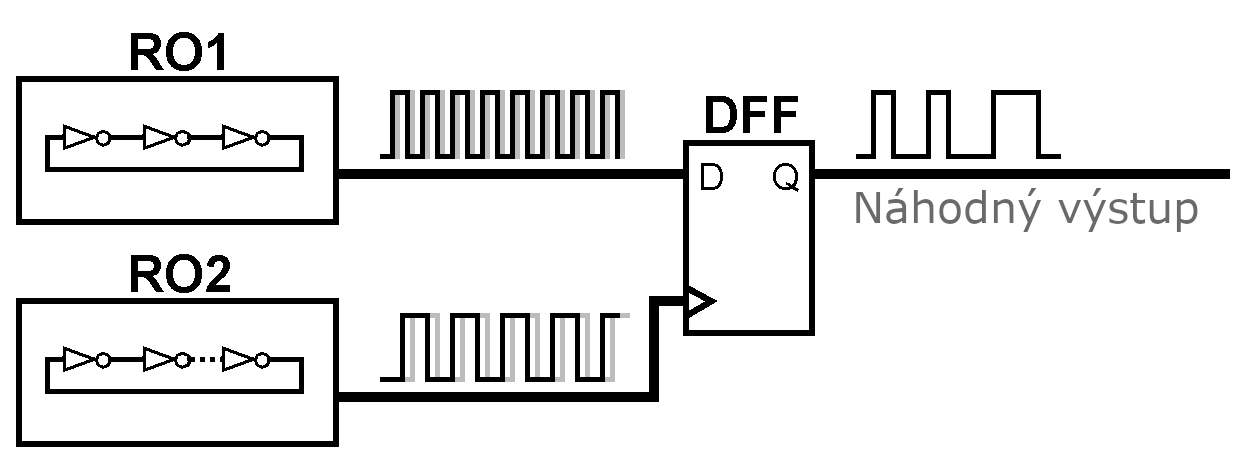
\includegraphics[width=.9\textwidth]{src/img1}
		\caption{TRNG na bázi jitteru z různě dlouhých kruhových oscilátorů}
		\label{_tag_img_jitter}
	\end{figure}
	
	\subsection{Metastabilita}
	
	Metastabilita v logických obvodech je stav, kdy se hodnota signálu nenachází v rozsahu pro logickou jedničku ani nulu („zakázaný“ / „nedefinovaný“ stav). Obvody, ve kterých se nachází takovýto signál, se mohou chovat nepředvídatelně a lze je tedy použít jako zdroj entropie.
	
	Do této kategorie patří \textit{Feedback Stabilized Metastable Latch Entropy Source} (FSMLES). Základní myšlenkou tohoto generátoru jsou dvě cyklicky zapojené negace, které se po přivedení napájení dostanou do jednoho ze dvou stavů (viz obrázek \ref{_tag_img_fsmles}). Protože jsou hradla stejná, měl by výsledný stav záležet pouze na šumu. Rychlým přiváděním a odváděním napájení by tedy teoreticky měl vzniknout rychlý a kvalitní zdroj entropie.
	
	Ve skutečnosti se ale takovéto zapojení bude vždy přiklánět k jednomu ze dvou stavů. Zjednodušeně řečeno je jedno hradlo silnější a vždy vyhraje. V praxi je toto řešeno dodatečnými obvody, které slabšímu hradlu pomohou. Podle Johnstona (zdroj \cite{z2}) na tomto principu funguje generace náhody v procesorech Intel pomocí instrukce \texttt{RDRAND}.
		
	\begin{figure}[ht]
		\centering
		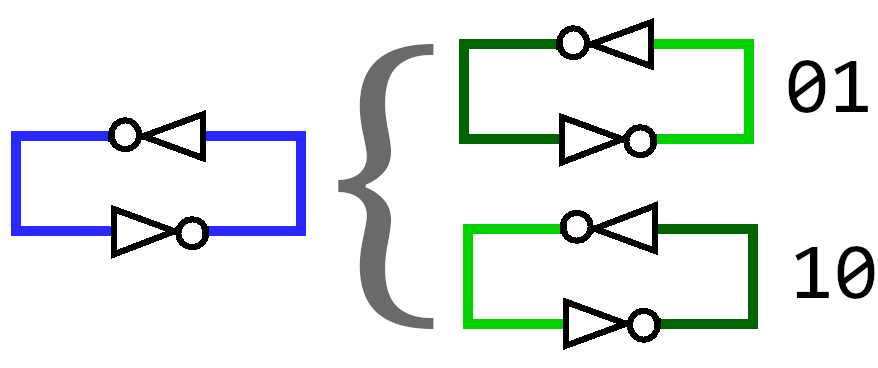
\includegraphics[width=.55\textwidth]{src/img2}
		\caption{Základ FSMLES}
		\label{_tag_img_fsmles}
	\end{figure}
		
	\section{Software CS-PRNG}

	\subsection{Blum Blum Shub}
	
	Algoritmus Blum Blum Shub generuje pseudonáhodná čísla pomocí vzorce: $$x_{n+1}=x_n^2 \bmod PQ$$, kde $P$, $Q$ jsou velká (2048 bitů a více) prvočísla a $x_0$ je počáteční stav, pro které platí:
	\begin{itemize}
		\item $P \neq Q$,
		\item $P \equiv 3 \pmod 4$,
		\item $Q \equiv 3 \pmod 4$,
		\item $x_0 \ge 2$ je nesoudělné s $P$ a $Q$.
	\end{itemize}
	Pseudonáhodný bit je pak určen jako parita $x_n$. Pro každý výstupní bit je tedy nutné znovu provést výpočet daný vzorcem.
	
	Toto je jeden z nejjednodušších, ale zároveň nejméně efektivních, kryptograficky bezpečných algoritmů pro generaci pseudonáhodných čísel. Důvodem je náročnost výpočtu uvedeného vzorce a určení počátečních hodnot. Efektivnější CS-PRNG jsou založeny na existujících kryptografických šifrách a hashovacích funkcích.

	\subsection{ChaCha}
	
	ChaCha je proudová šifra, kterou lze použít jako generátor pseudonáhodných čísel. Jedná se o nástupce a modifikaci šifry Salsa20. Vstup algoritmu si lze představit jako tabulku o rozměru $4\times4$, kde velikost jedné buňky je 32 bitů. Osm buněk tabulky tvoří klíč (256 bitů), za který jsou v tomto případě dosazena entropická data. Čtyři buňky jsou pak konstantní a zbytek je čítač a nonce.
	
	Po dobu dvaceti kol (rund) jsou s buňkami v tabulce prováděny určité sekvence operací s tím, že tabulka je rozdělena na čtyři čtveřice buněk a pro každou čtveřici je sekvence provedena zvlášť. V lichých kolech se jedná o sloupce a v sudých kolech o diagonály tabulky (viz obrázek \ref{_tag_img_chacha}).
	
	\begin{figure}[ht]
		\centering
		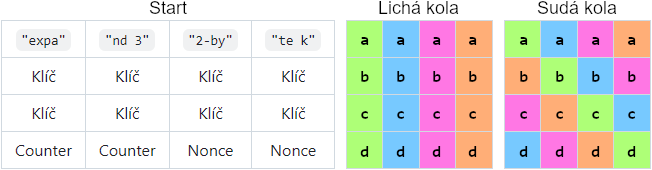
\includegraphics[width=\textwidth]{src/img4}
		\caption{ChaCha tabulka}
		\label{_tag_img_chacha}
	\end{figure}
	
	Šifra je typu ARX, jediné používané operace jsou tedy sčítání (modulo $2^{32}$), bitová rotace a XOR. Konkrétní prováděné operace v každém kole popisuje obrázek \ref{_tag_img_chachastep}. Po dvaceti kolech je obsahem tabulky 512 pseudonáhodných bitů. Pro generaci dalších 512 bitů se inkrementuje čítač a algoritmus dvaceti kol se opakuje. Po přetečení čítače nebo změně klíče je nutno změnit nonce.
	
	\begin{figure}[ht]
		\centering
		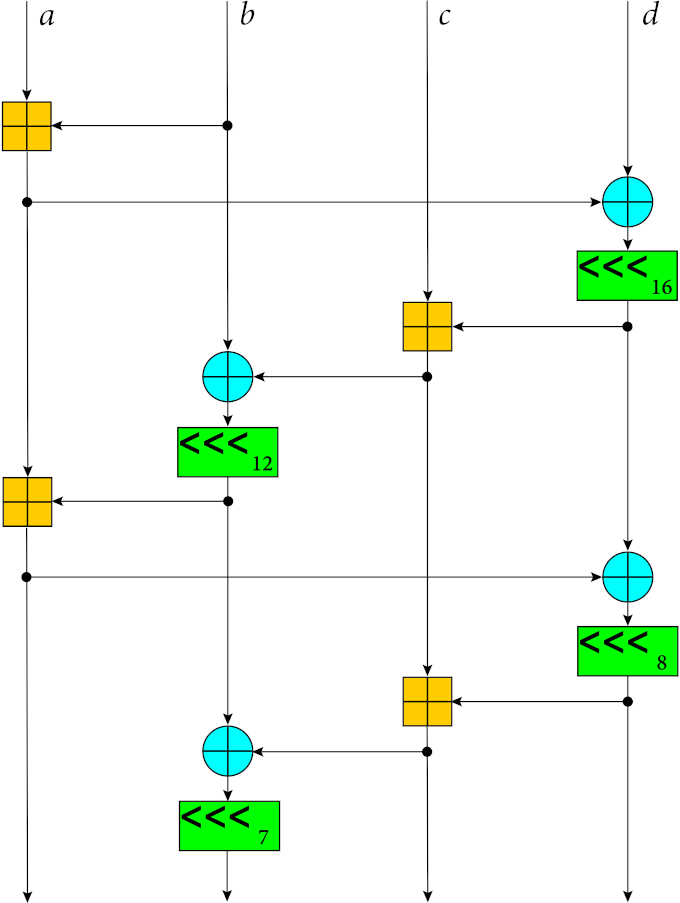
\includegraphics[width=.5\textwidth]{src/img3}
		\caption{ChaCha – čtvrtina každého kola \cite{z5}}
		\label{_tag_img_chachastep}
	\end{figure}
		
	\subsection{AES v režimu CTR}
	
	Šifra AES, a blokové šifry obecně, mohou pracovat v několika režimech. Režim \textit{Counter} (CTR) z blokové šifry v podstatě dělá šifru proudovou: Do každého bloku vstupuje klíč, nonce a čítač. Čítač je inkrementován pro každý blok a trojice (klíč, nonce, čítač) by se nikdy neměla opakovat. Pro potřeby PRNG jsou za klíč dosazena entropická data a výstup bloku je již brán jako pseudonáhodné bity. Pro potřeby šifrování jsou výstupní bity „XORovány“ s částí plaintext zprávy. Jedná se tedy o stejné schéma jako u šifry ChaCha.
	
	Po dobu několika kol (rund) jsou na interním stavu šifry prováděny určité operace a po posledním kole je interní stav roven výsledku. Šifra přijímá klíč o velikosti 128/192/256 bitů, jehož velikost určuje počet kol na 10/12/14. Z klíče je pomocí speciální funkce vytvořen takový počet \textit{rundovních} klíčů, které odpovídají počtu kol, a před každým kolem je interní stav šifry XORován s aktuálním rundovním klíčem.
	
	Interní stav šifry lze reprezentovat tabulkou o rozměru $4\times4$, kde velikost jedné buňky je 8 bitů. Počáteční stav je nonce a čítač, které tedy dohromady zabírají 128 bitů, a doporučuje se použít 96 bitů pro nonce a 32 bitů pro čítač.
	
	V každém kole je nejprve provedena substituce buněk podle veřejně známé tabulky. Následně jsou buňky v jednotlivých řádcích rotovány doleva o $n$ pozic, kde $n=rowNumber-1$ (první řádek se nezmění). Posledním krokem, který se neprovádí v posledním kole, je rozptýlení sloupců: Každý sloupec je vynásoben speciální maticí, kde je ale „součet“ jednotlivých prvků definován jako XOR a na násobení je aplikováno modulo.% $2^8$.
		
	Šifra AES je standardizována a díky existujícím speciálním CPU instrukcím je velmi rychlá. Oproti tomu ChaCha je méně náchylná na útoky postranním kanálem a může být rychlejší na hardwaru, který AES nativně nepodporuje.
	
	Šifra AES se také používá jako extraktor entropie, konkrétně v režimu CBC-MAC. Vstupní plaintext zprávou jsou v tomto případě surová entropická data o délce přímo úměrné počtu AES bloků ($128\cdot nBlocks$ bitů). Počáteční hodnota IV je nulová a klíčem může být libovolné číslo nezávislé na vstupních datech. Výstupem je 128bitový tag, který obsahuje bity s kvalitnější náhodou.
	
	\section{Dostupné implementace}
	
	\subsection{Instrukce \texttt{RDRAND} a \texttt{RDSEED}}
	
	Architektury x86 obsahují instrukce \texttt{RDRAND} a \texttt{RDSEED}, které naplní určitý registr náhodnými bity, jež jsou vhodné pro kryptografická použití.
	
	Procesory Intel používají zdroj entropie na principu metastability, extraktorem entropie je AES CBC-MAC a generátorem je AES CTR. Instrukce \texttt{RDRAND} čerpá náhodné bity z generátoru. \textit{Reseed} generátoru (dodání čerstvé entropie) je prováděn automaticky. Instrukce \texttt{RDSEED} čerpá bity přímo z extraktoru entropie a XORuje je s bity generátoru. Je vhodná např. pro generování klíčů delších než 128 bitů nebo pro reseed vlastního PRNG.
	
	\subsection{Linux: \texttt{/dev/urandom}}
	
	Na unixových systémech je \texttt{/dev/urandom} soubor reprezentující znakové zařízení, který obsahuje náhodné bity. OS Linux získává entropické bity z řady zdrojů (uživatelská aktivita, časování přerušení) a pseudonáhodné bity z nich dělá pomocí hashovací funkce.
	
	Existuje také soubor \texttt{/dev/random}, který se snaží určit svou hodnotu entropie a nevrací bity, je-li hodnota příliš nízká. Určování hodnoty entropie ale není obecně spolehlivé a není proto důvod používat \texttt{/dev/random} namísto \texttt{/dev/urandom}.
	
	\subsection{Náhoda v programovacích jazycích}
	
	Při programování kryptografické aplikace není bezpečné používat běžné funkce pro generaci náhodných čísel. Je potřeba použít specializované funkce nebo knihovny, např. v jazyce Python nepoužívat funkci \texttt{random.getrandbits}, ale funkci \texttt{os.urandom}, případně balík \texttt{secrets} nebo přímo balík \texttt{rdrand}.
		
	% Zdroje
	\null\vfill\section*{Použité zdroje}\printbibliography[heading=none]
	
\end{document}
